\chapter{Correlation}
\label{ch:correlation}

In this chapter we will dive much deeper into understanding the core
algorithms in the Stereo Pipeline.  We start with an overview of the
five stages of stereo reconstruction.  Then we move into an in-depth
discussion and exposition of the various correlation algorithms.

The goal of this chapter is to build an intuition for the stereo
correlation process.  This will help users to identify unusual results
in their \acp{DEM} and hopefully eliminate them by tuning various
parameters in the \texttt{stereo.default} file.  For scientists and
engineers who are using \acp{DEM} produced with the Stereo Pipeline, this
chapter may help to answer the question, ``What is the Stereo Pipeline
doing to the raw data to produce this \ac{DEM}?''

A related question that is commonly asked is, ``How accurate is a \ac{DEM}
produced by the Stereo Pipeline?''  This chapter does not yet address
matters of accuracy and error, however we have several efforts underway
to quantify the accuracy of Stereo Pipeline-derived \acp{DEM}, and will be
publishing more information about that shortly.  Stay tuned.

The entire stereo correlation process, from raw input images to a
point cloud or DEM, can be viewed as a multistage pipeline as depicted
in Figure~\ref{fig:asp}, and detailed in the following sections.

\begin{figure}[tb]
  \centering
  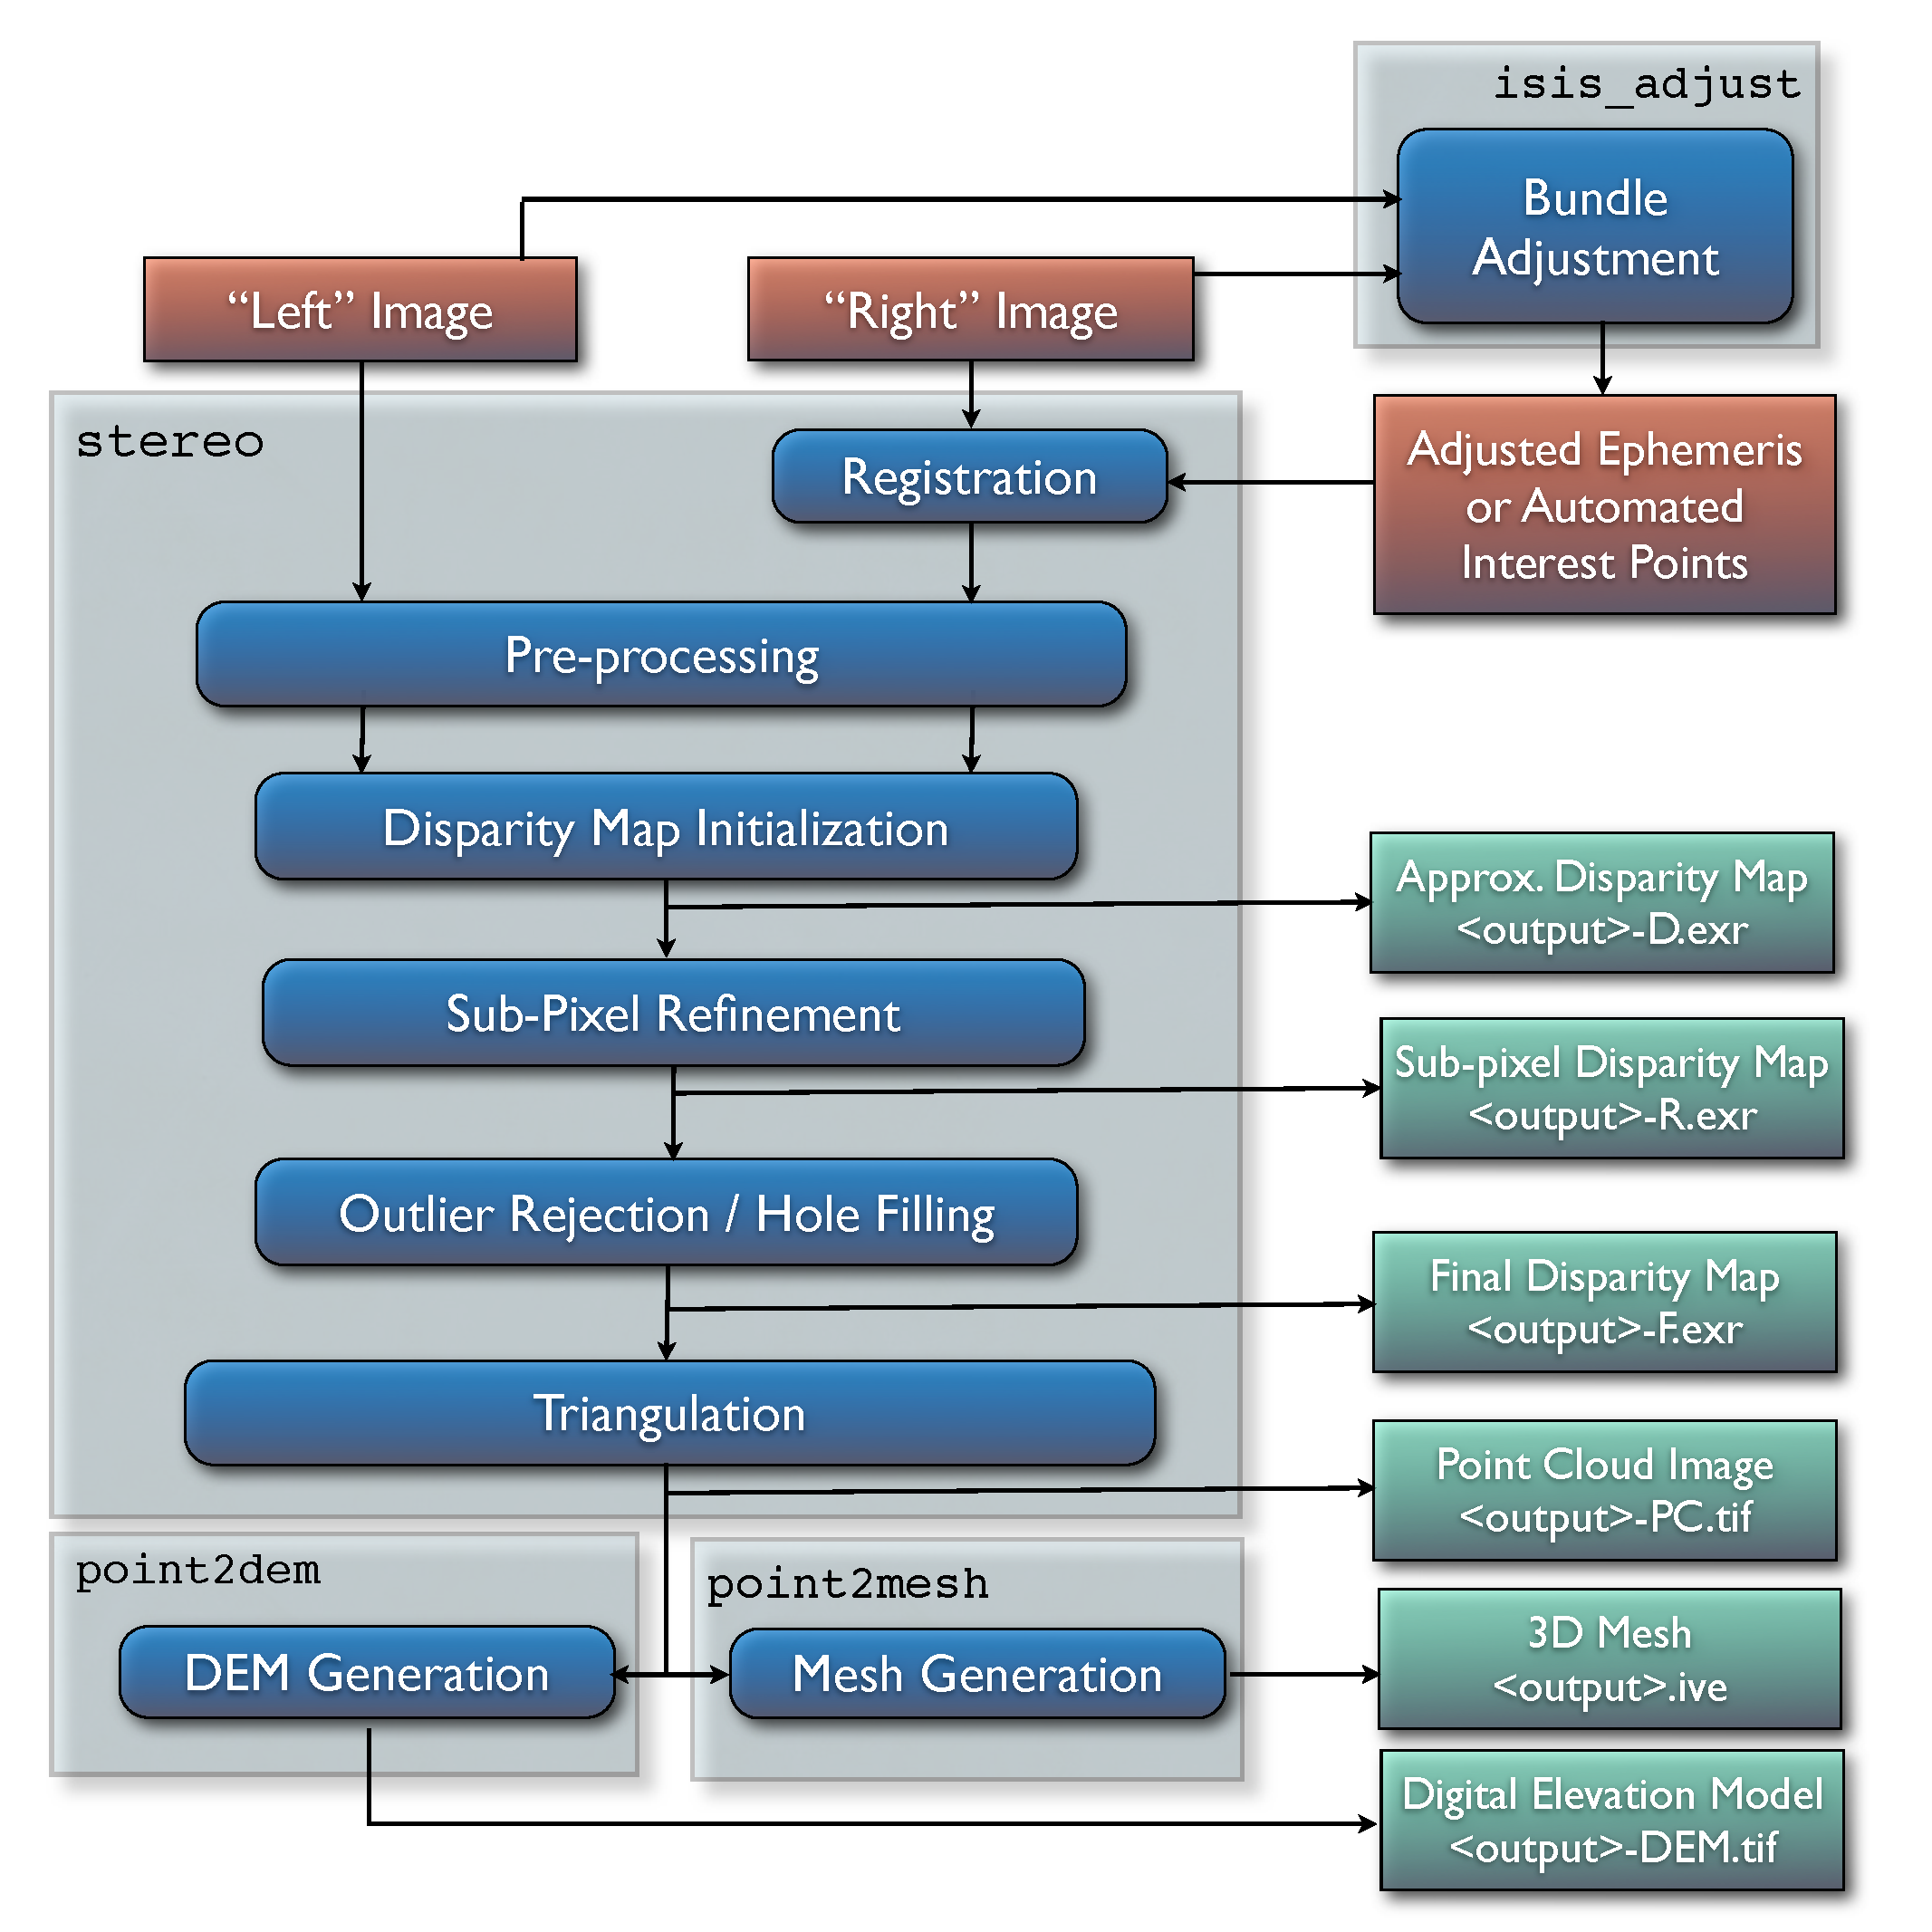
\includegraphics[width=13cm]{images/asp}
  \caption{Flow of data through the Stereo Pipeline.}
  \label{fig:asp}
\end{figure}

\section{Pre-processing}

The first optional (but recommended) step in the process is least
squares Bundle Adjustment, which is described in detail in
Chapter~\ref{ch:bundle_adjustment}.

Next, the left and right images are roughly aligned using one of three
methods: (1) a homography transform of the right image based on
automated tie-point measurements, (2) a 3D rotation that achieves
epipolar rectification {\it(only implemented for Pinhole sessions for
  missions like MER or K10)} or (3) map projection of both the left
and right images using the \ac{ISIS} \texttt{cam2map} command or
through \texttt{gdal\_translate} for Digital Globe and GeoEye images.
The first two options can be applied automatically by the stereo
pipeline when the \texttt{alignment-method} variable in the
\texttt{stereo.default} file is set to \texttt{HOMOGRAPHY} or
\texttt{EPIPOLAR}.

The latter option, running {\tt cam2map}, {\tt cam2map4stereo.py}, or
{\tt gdal\_translate} must be carried out by the user prior to
invoking the {\tt stereo} command.  Map projecting the images using
\ac{ISIS} eliminates any unusual distortion in the image due to the
unusual camera acquisition modes (e.g. pitching ``ROTO'' maneuvers
during image acquisition for \ac{MOC}, or highly elliptical orbits and
changing line exposure times for the \acl{HRSC}, \acs{HRSC}).  It also
eliminates some of the perspective differences in the image pair that
are due to large terrain features by taking the existing low-res
terrain model into account (e.g. the \acl{MOLA}, \acs{MOLA};
\acl{LOLA}, \acs{LOLA}; \acl {NED}, \acs {NED}; or \acl{ULCN},
\acs{ULCN}, 2005 models).

In essence, map projecting the images results in a pair of very
closely matched images that are as close to ideal as possible given
existing information. This leaves only small perspective differences
in the images, which are exactly the features that the stereo
correlation process is designed to detect.

For this reason, we recommend map projection for pre-alignment of most
stereo pairs. Its only cost is longer triangulation times as more math
must be applied to work back through the transforms applied to the images. In
either case, the pre-alignment step is essential for performance
because it ensures that the disparity search space is bounded to a
known area.  In both cases, the effects of pre-alignment are taken
into account later in the process during Triangulation, so you do not
need to worry that pre-alignment will compromise the geometric
integrity of your \ac{DEM}.

In some cases the pre-processing step may also normalize the pixel
values in the left and right images to bring them into the same
dynamic range.  Various options in the {\tt stereo.default} file
affect whether or how normalization is carried out, including
\texttt{individually-normalize} and
\texttt{force-use-entire-range}.  Although the defaults work in
most cases, the use of these normalization steps can vary from data
set to data set, so we recommend you refer to the examples in Chapter
\ref{ch:examples} to see if these are necessary in your use case.

Finally, pre-processing can perform some filtering of the input
images (as determined by \\ \texttt{prefilter-mode}) to reduce noise
and extract edges in the images.  When active, these filters apply
a kernel with a sigma of \texttt{prefilter-kernel-width} pixels
that can improve results for noisy images (\texttt{prefilter-mode}
must be chosen carefully in conjunction with \texttt{cost-mode},
see Appendix~\ref{ch:stereodefault}).  The pre-processing modes
that extract image edges are useful for stereo pairs that do not
have the same lighting conditions, contrast, and absolute brightness
\citep{Nishihara84practical}.  We recommend that you use the defaults
for these parameters to start with, and then experiment only if
your results are sub-optimal.

\section{Disparity Map Initialization}

Correlation is the process at the heart of the Stereo Pipeline.  It is
a collection of algorithms that compute correspondences between pixels
in the left image and pixels in the right image.  The map of these
correspondences is called a {\em disparity map}.  You can think of a
disparity map as an image whose pixel locations correspond to
the pixel $(u,v)$ in the left image, and whose pixel values
contain the horizontal and vertical offsets $(d_u, d_v)$ to the
matching pixel in the right image, which is $(u+d_u, v+d_v)$.

The correlation process attempts to find a match for every pixel in
the left image. The only pixels skipped are those marked invalid in
the mask images. For large images (e.g. from \ac{HiRISE}, \acl{LROC},
\acs{LROC}, or WorldView), this is very expensive computationally, so
the correlation process is split into two stages.  The disparity map
initialization step computes approximate correspondences using a
pyramid-based search that is highly optimized for speed, but trades
resolution for speed. The results of disparity map initialization are
integer-valued disparity estimates.  The sub-pixel refinement step
takes these integer estimates as initial conditions for an iterative
optimization and refines them using the algorithm discussed in the
next section.

We employ several optimizations to accelerate disparity map
initialization: (1) a box filter-like accumulator that reduces
duplicate operations during correlation \citep{Sun02rectangular}; (2) a
coarse-to-fine pyramid based approach where disparities are estimated
using low resolution images, and then successively refined at higher
resolutions; and (3) partitioning of the disparity search space into
rectangular sub-regions with similar values of disparity determined in
the previous lower resolution level of the
pyramid \citep{Sun02rectangular}.

\begin{figure}[bt]
  \centering
  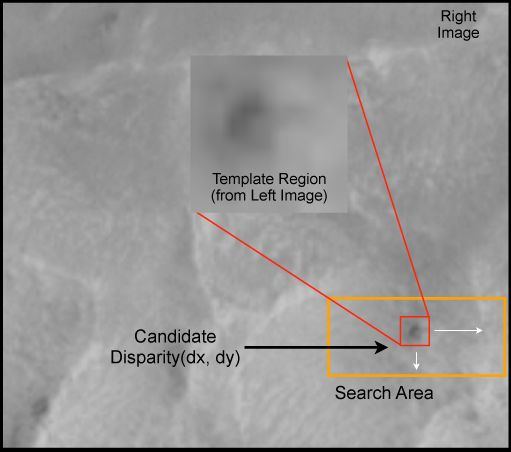
\includegraphics[width=13cm]{images/correlation/correlation}
  \caption{The correlation algorithm in disparity map initialization
    uses a sliding template window from the left image to find the
    best match in the right image.  The size of the template window
    can be adjusted using the \texttt{H\_KERN} and \texttt{V\_KERN} parameters in the
    \texttt{stereo.default} file, and the search range can be adjusted
    using the \{\texttt{H},\texttt{V}\}\texttt{\_CORR\_}\{\texttt{MIN}/\texttt{MAX}\} parameters.}
  \label{fig:correlation_window}
\end{figure}

Naive correlation itself is carried out by moving a small, rectangular
template window from the from left image over the specified search
region of the right image, as in Figure~\ref{fig:correlation_window}.
The ``best'' match is determined by applying a cost function that
compares the two windows. The location at which the window evaluates
to the lowest cost compared to all the other search locations is
reported as the disparity value. The \texttt{cost-mode} variable allows you
to choose one of three cost functions, though we recommend normalized
cross correlation \citep{Menard97:robust}, since it is most robust to
slight lighting and contrast variations between a pair of
images. Try the others if you need more speed at the cost of quality.

Our implementation of pyramid correlation is a little unique in that
it is actually split into two levels of pyramid searching. There is a
\texttt{\textit{output\_prefix}-D\_sub.tif} disparity image that is
computed from the greatly reduced input images \texttt{*-L\_sub.tif}
and \texttt{\textit{output\_prefix}-R\_sub.tif}. Those ``sub'' images
have their size chosen so that their area is around 2.25 mega pixels,
a size that is easily viewed on the screen unlike the raw source
imagery. The low resolution disparity image then defines the per
thread search range of the higher resolution disparity,
\texttt{\textit{output\_prefix}-D.tif}.

This solution is imperfect but comes from our model of multithreaded
processing. ASP processes individual tiles of the output disparity
in parallel. The smaller the tiles, the easier it is to distribute
evenly among the CPU cores. The size of the tile unfortunately
limits the max number of pyramid levels we can process. We've struck
a balance where every 1024 by 1024 pixel area is processed individually
in a tile. This practice allows only 5 levels of pyramid processing.
With the addition of the second tier of pyramid searching with
\texttt{\textit{output\_prefix}-D\_sub.tif}, we are allowed to
process beyond that limitation.

Any large failure in
the low resolution disparity image will be detrimental to the
performance of the higher resolution disparity. In the event that the
low resolution disparity is completely unhelpful, it can be skipped by
adding \texttt{corr-seed-mode 0} in the \texttt{stereo.default}
file. This should only be considered in cases where the texture in an
image is completely lost when subsampled. An example would be
satellite imagery of fresh snow in the arctic.

An alternative to computing \texttt{\textit{output\_prefix}-D.tif}
from sub-sampled images (\texttt{corr-seed-mode 1}) or skipping it
altogether (\texttt{corr-seed-mode 0}), is to compute it from a
lower-resolution DEM of the area (\texttt{corr-seed-mode 2}). In this
situation, the low-resolution DEM needs to be specified together with its estimated
error. See section \ref{corr_section} for more detailed information as
to how to specify these options. In our experiments, if the input DEM
has a resolution of 1 km, a good value for the DEM error is about 10 m,
or higher if the terrain is very variable.

\subsection{Debugging Disparity Map Initialization}

Never will all pixels be successfully matched during stereo
matching. Though a good chunk of the image should be correctly
processed. If you see large areas where matching failed, this could be
due to a variety of reasons:

\begin{itemize}
\item In regions where the images do not overlap, there should be no
  valid matches in the disparity map.
\item Match quality may be poor in regions of the images that have
  different lighting conditions, contrast, or specular properties of
  the surface.
\item Areas that have image content with very little texture or
  extremely low contrast may have an insufficient signal to noise
  ratio, and will be rejected by the correlator.
\item Areas that are highly distorted due to different image
  perspective, such as crater and canyon walls, may exhibit poor
  matching performance. This could also be due to failure of the
  preprocessing step in aligning the images. The correlator can not
  match images that are rotated differently from each other or have
  different scale/resolution.
\end{itemize}

Bad matches, often called ``blunders'' or ``artifacts'' are also
common, and can happen for many of the same reasons listed above.  The
Stereo Pipeline does its best to automatically detect and eliminate
these blunders, but the effectiveness of these outlier rejection
strategies does vary depending on the quality of the input imagery.

When tuning up your {\tt stereo.default} file, you will find that
it is very helpful to look at the raw output of the disparity map
initialization step.  This can be done using the {\tt disparitydebug}
tool, which converts the \texttt{\textit{output\_prefix}-D.tif}
file into a pair of normal images that contain the horizontal and
vertical components of disparity.  You can open these in a standard
image viewing application and see immediately which pixels were
matched successfully, and which were not. Stereo matching blunders
are usually also obvious when inspecting these images.  With a good
intuition for the effects of various {\tt stereo.default} parameters
and a good intuition for reading the output of {\tt disparitydebug},
it is possible to quickly identify and address most problems.

\section{Sub-pixel Refinement}
\label{sec:subpixel}

Once disparity map initialization is complete, every pixel in the
disparity map will either have an estimated disparity value, or it
will be marked as invalid.  All valid pixels are then adjusted in the
sub-pixel refinement stage based on the \texttt{subpixel-mode}
setting. % Subpixel refinement is not additive step.

The first mode is parabola-fitting sub-pixel refinement
(\texttt{subpixel-mode 1}).  This technique fits a 2D parabola to
points on the correlation cost surface in an 8-connected neighborhood
around the cost value that was the ``best'' as measured during
disparity map initialization. The parabola's minimum can then be
computed analytically and taken as as the new sub-pixel disparity
value.

This method is easy to implement and extremely fast to compute, but it
exhibits a problem known as pixel-locking: the sub-pixel disparities
tend toward their integer estimates and can create noticeable ``stair
steps'' on surfaces that should be smooth
\citep{Stein06:attenuating,Szeliski03sampling}.  See
e.g. Figure~\ref{fig:parabola_subpixel}. Furthermore, the parabola
subpixel mode is not capable of refining a disparity estimate by more
than one pixel, so although it produces smooth disparity maps, these
results are not much more accurate than the results that come out of
the disparity map initialization in the first place.  However, the
speed of this method makes it very useful as a ``draft'' mode for
quickly generating a \ac{DEM} for visualization (i.e. non-scientific)
purposes. It is also beneficial in the event that a user will simply
downsample their DEM after generation in Stereo Pipeline.

\begin{figure}[tb]
\centering
  \subfigure[{\tt Left Image}]{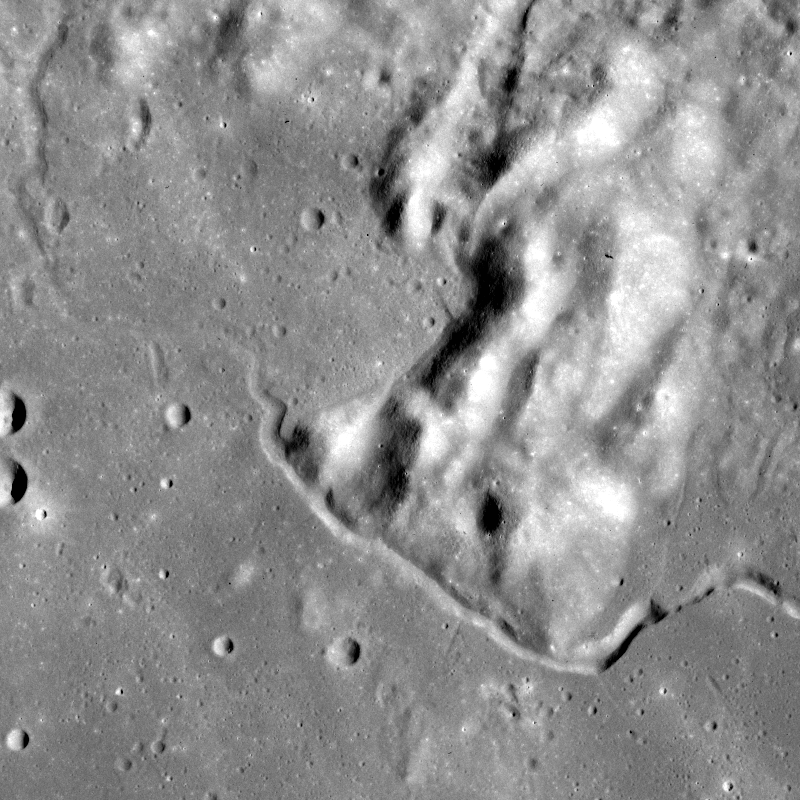
\includegraphics[width=2in]{images/correlation/sub4-AS15-M-1134_crop.png}\label{fig:left_input_image}}
  \subfigure[{\tt Parabola Subpixel Mode}]{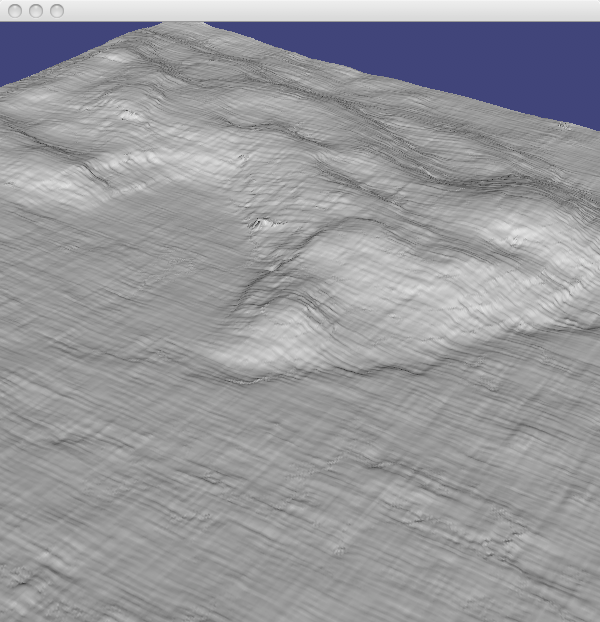
\includegraphics[width=2in]{images/correlation/3D_mode0.png}\label{fig:parabola_subpixel}}
  \subfigure[{\tt Bayes EM Subpixel Mode}]{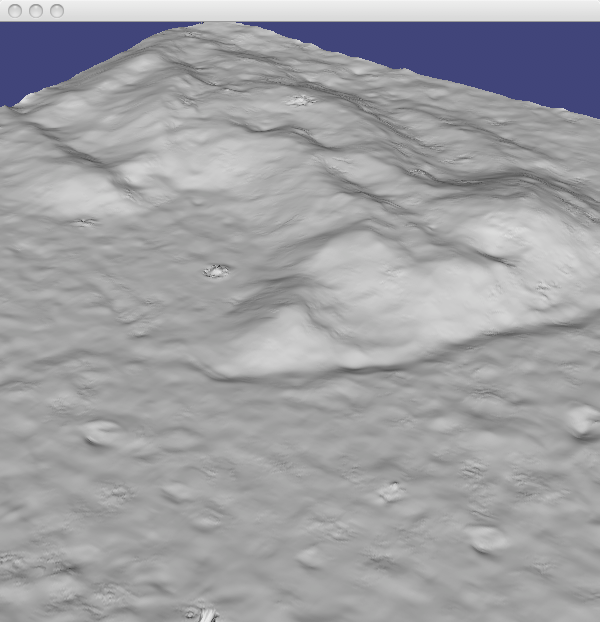
\includegraphics[width=2in]{images/correlation/3D_mode3.png}}

  \subfigure[{\tt Right Image}]{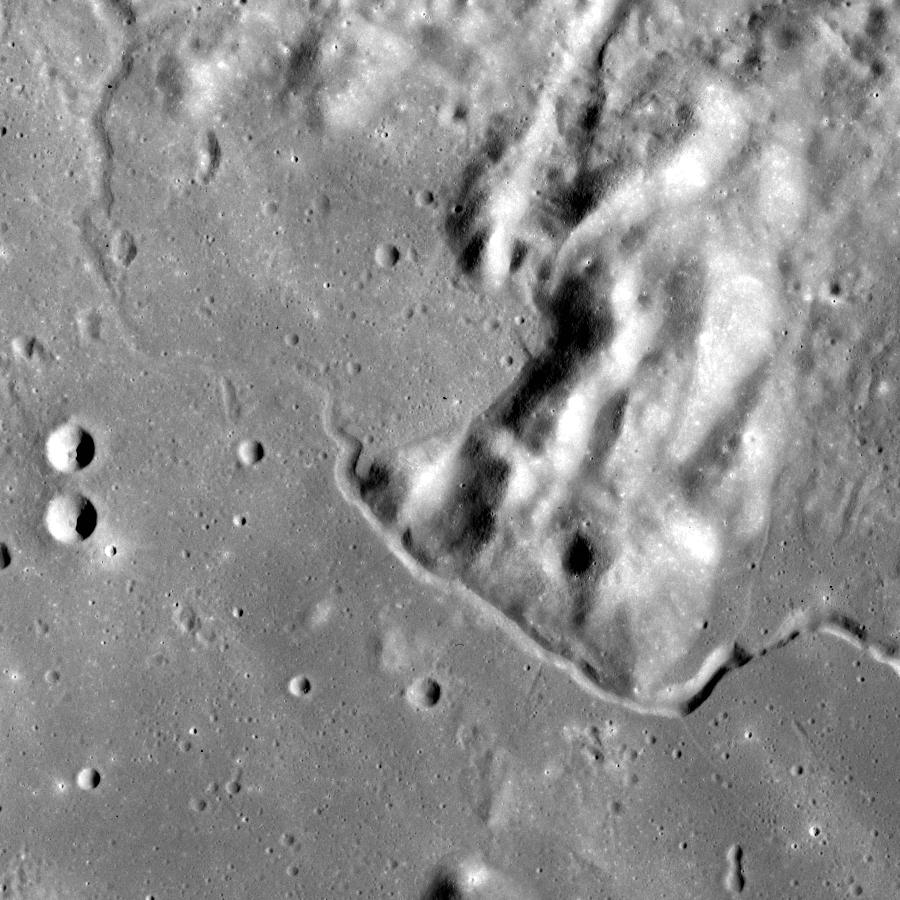
\includegraphics[width=2in]{images/correlation/sub4-AS15-M-1135_crop.png}\label{fig:right_input_image}}
  \subfigure[{\tt Parabola Hillshade}]{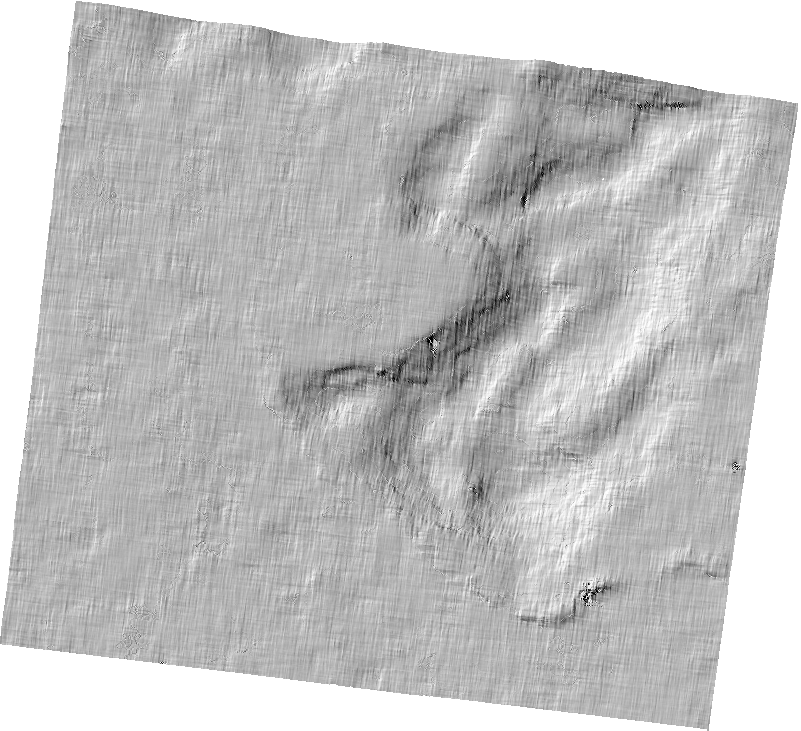
\includegraphics[width=2in]{images/correlation/hillshade_mode0.png}}
  \subfigure[{\tt Bayes EM Hillshade}]{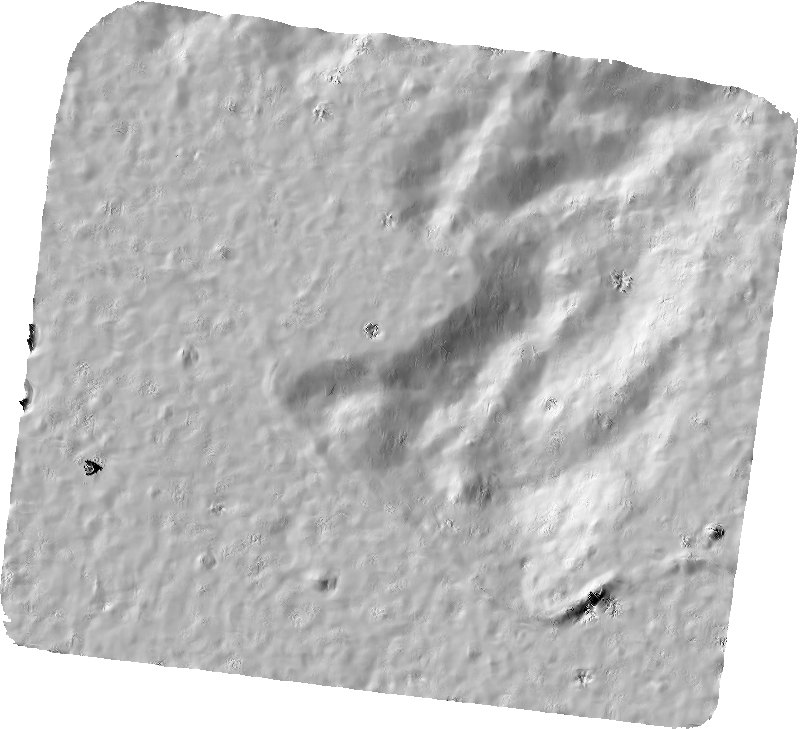
\includegraphics[width=2in]{images/correlation/hillshade_mode3.png}}

\caption{Left: Input images.  Center: results using the parabola draft
  subpixel mode (\texttt{subpixel-mode = 1}). Right: results using the Bayes
  EM high quality subpixel mode (\texttt{subpixel-mode = 2}).}
\label{fig:parabola_results}
\end{figure}

For high quality results, we recommend \texttt{subpixel-mode 2}:
the Bayes EM weighted affine adaptive window correlator.  This
advanced method produces extremely high quality stereo matches that
exhibit a high degree of immunity to image noise.  For example
Apollo Metric Camera images are affected by two types of noise
inherent to the scanning process: (1) the presence of film grain
and (2) dust and lint particles present on the film or scanner.
The former gives rise to noise in the \ac{DEM} values that wash out real
features, and the latter causes incorrect matches or hard to detect
blemishes in the \ac{DEM}.  Attenuating the effect of these scanning
artifacts while simultaneously refining the integer disparity map
to sub-pixel accuracy has become a critical goal of our system, and
is necessary for processing real-world data sets such as the Apollo
Metric Camera data.

The Bayes EM subpixel correlator also features a deformable template
window from the left image that can be rotated, scaled, and translated
as it zeros in on the correct match in the right image.  This
adaptive window is essential for computing accurate matches on crater
or canyon walls, and on other areas with significant perspective
distortion due to foreshortening.

This affine-adaptive behavior is based on the Lucas-Kanade template
tracking algorithm, a classic algorithm in the field of computer
vision \citep{Baker04:lucas-kanade}.  We have extended this technique;
developing a Bayesian model that treats the Lucas-Kanade parameters
as random variables in an Expectation Maximization (EM) framework.
This statistical model also includes a Gaussian mixture component
to model image noise that is the basis for the robustness of our
algorithm.  We will not go into depth on our approach here, but we
encourage interested readers to read our papers on the topic
\citep{nefian:bayes_em, broxton:isvc09}.

However we do note that, like the computations in the disparity map
initialization stage, we adopt a multi-scale approach for sub-pixel
refinement. At each level of the pyramid, the algorithm is initialized
with the disparity determined in the previous lower resolution level
of the pyramid, thereby allowing the subpixel algorithm to shift the
results of the disparity initialization stage by many pixels if a better
match can be found using the affine, noise-adapted window.  Hence,
this sub-pixel algorithm is able to significantly improve upon the
results to yield a high quality, high resolution result.

\section{Triangulation}

When running an ISIS session, the Stereo Pipeline uses geometric
camera models available in \ac{ISIS} \citep{anderson08:isis}.  These
highly accurate models are customized for each instrument that
\ac{ISIS} supports.  Each \ac{ISIS} ``cube'' file contains all of the
information that is required by the Stereo Pipeline to find and use
the appropriate camera model for that observation.

Other sessions such as DG (\textit{Digital Globe}) or Pinhole, require that
their camera model be provided as additional arguments to the
\texttt{stereo} command. Those camera models come in the form of an
XML document for DG and as \texttt{*.pinhole, *.tsai, *.cahv,
  *.cahvor} for Pinhole sessions. Those files must be the third and
forth arguments or immediately follow after the 2 input images for
\texttt{stereo}.

\begin{figure}[h]
\centering
  \subfigure[{\tt Framing Camera Model}]{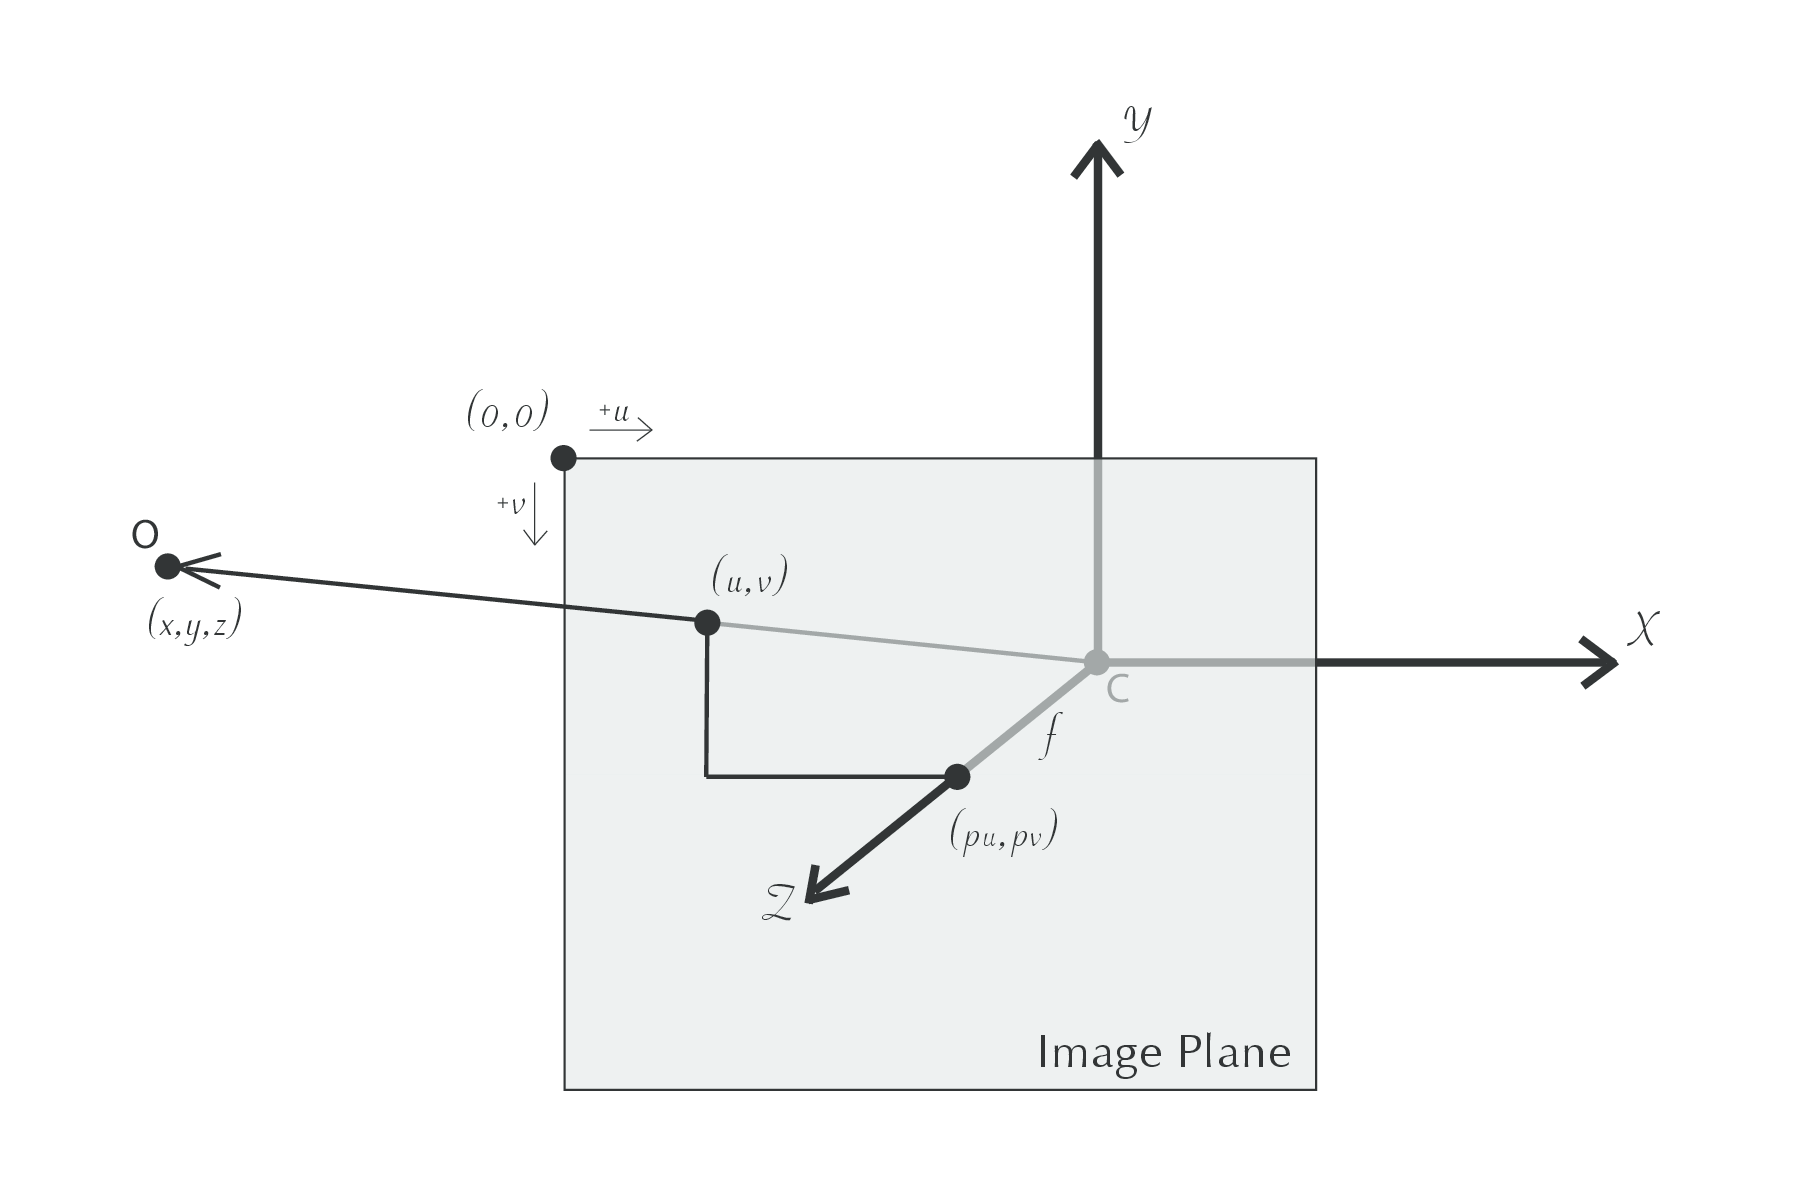
\includegraphics[width=3in]{images/correlation/pinhole_model}\label{fig:framing}}
  \subfigure[{\tt Pushbroom Camera Model}]{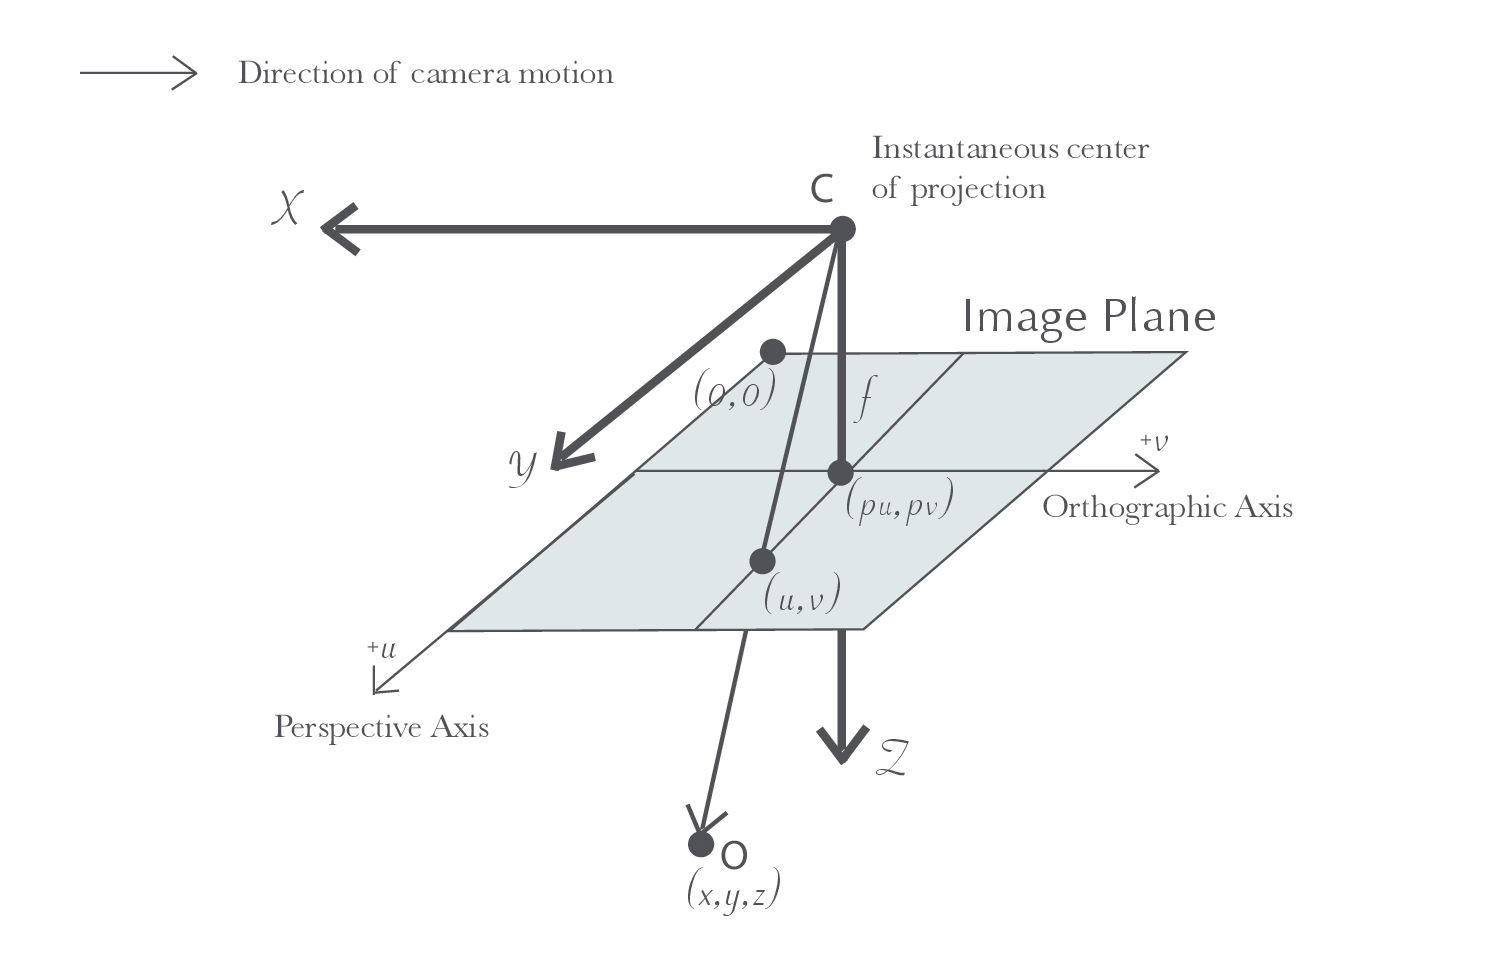
\includegraphics[width=3in]{images/correlation/linescan_model}\label{fig:linescan}}
\caption{Most remote sensing cameras fall into two generic categories
  based on their basic geometry.  Framing cameras (left) capture an
  instantaneous two-dimensional image.  Linescan cameras (right)
  capture images one scan line at a time, building up an image over
  the course of several seconds as the satellite moves through the
  sky.}
\label{fig:camera_models}
\end{figure}

\ac{ISIS} camera models account for all aspects of camera geometry,
including both intrinsic (i.e. focal length, pixel size, and lens
distortion) and extrinsic (e.g. camera position and orientation)
camera parameters.  Taken together, these parameters are sufficient to
``forward project'' a 3D point in the world onto the image plane of
the sensor.  It is also possible to ``back project'' from the camera's
center of projection through a pixel corresponding to the original 3D
point.

\begin{figure}[tb]
  \centering
  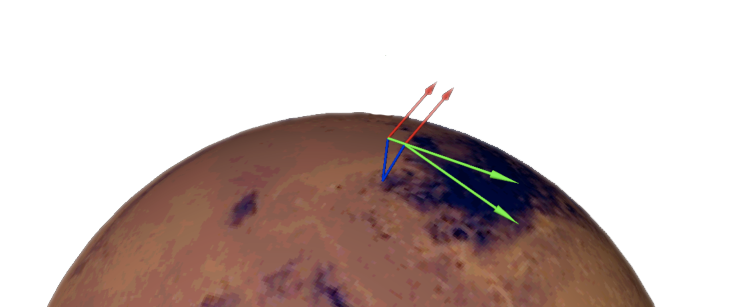
\includegraphics[width=12cm]{images/correlation/triangulation}
  \caption{Once a disparity map has been generated and refined, it can
    be used in combination with the geometric camera models to compute
    the locations of 3D points on the surface of Mars.  This figure
    shows the position (at the origins of the red, green, and blue vectors) and
	orientation of the Mars Global Surveyor at
    two points in time where it captured images in a stereo pair.}
  \label{fig:triangulation}
\end{figure}

Notice, however, that forward and back projection are not symmetric
operations.  One camera is sufficient to ``image'' a 3D point onto a
pixel located on the image plane, but the reverse is not true.  Given
only a single camera and a pixel location $x = (u,v)$ that is the
image of an unknown 3D point $P = (x,y,z)$, it is only possible to
determine that $P$ lies somewhere along a ray that emanates from the
camera's center of projection through the pixel location $x$ on the
image plane (see Figure~\ref{fig:camera_models}).

Alas, once images are captured, the route from image pixel back to 3D
points in the real world is through back projection, so we must bring
more information to bear on the problem of uniquely reconstructing our
3D point.  In order to determine $P$ using back projection, we need
{\em two} cameras that both contain pixel locations $x_1$ and $x_2$
where $P$ was imaged.  Now, we have two rays that converge on a point
in 3D space (see Figure~\ref{fig:triangulation}). The location where
they meet must be the original location of $P$.

In practice, the two rays rarely intersect perfectly because any
slight error in the camera position or pointing information will
effect the rays' positions as well.  Instead, we take the {\em closest
  point of intersection} of the two rays as the location of point
$P$.

Additionally, the actual distance between the rays at this point is an
interesting and important error metric that measures how
self-consistent our two camera models are for this point.  You will
learn in the next chapter that this information, when computed and
averaged over all reconstructed 3D points, can be a valuable statistic
for determining whether to carry out bundle adjustment. Distance
between the two rays at their closest intersection is recorded in the
fourth channel of the point cloud file,
\texttt{\textit{output-prefix}-PC.tif}. This information can be
brought to the same perspective as the output DEM by using the
\textit{-\/-error} argument on the \texttt{point2dem} command.

This error in the triangulation, the distance between two rays,
\emph{is not the true accuracy of the DEM}. It is only another
indirect measure of quality. A DEM with high triangulation error
is always bad and should have its images bundle adjusted. A DEM
with low triangulation error is at least self consistent but could
still be bad. A map of the triangulation error should only be
interpreted as a relative measurement. Where small areas are found
with high triangulation error came from correlation mistakes and
large areas of error came from camera model inadequacies.
